\documentclass{article}
\usepackage[utf8]{inputenc}
\usepackage{amsmath, amsthm, amssymb}
\usepackage{enumitem}
\usepackage{mathtools}
\usepackage[margin=1in]{geometry}

\usepackage{hyperref}
\usepackage{subcaption}

\usepackage{fourier} % math & rm
\usepackage[scaled=0.875]{helvet} % ss

\newcommand{\code}{\texttt}

\title{Udacity SDC Nanodegree Project 1\\
Finding Lane Lines on the Road}
\author{Alexander Reynolds\\
    \href{mailto:ar@reynoldsalexander.com}{ar@reynoldsalexander.com}}
\date{June 1, 2017}

\begin{document}
\maketitle

%%%%%%%%%%%%%%%%%%%%%%%%%%%%%%%%%%%%%%%%%%%%%%%%%%%%%%
\section{Introduction}

This project is the first of many for the Udacity Self-Driving Car Nanodegree. The project introduces \code{OpenCV} on \code{Python}, and the task is to produce a pipeline that finds lane lines on still images and video of a car driving in lanes.

%%%%%%%%%%%%%%%%%%%%%%%%%%%%%%%%%%%%%%%%%%%%%%%%%%%%%%

\section{Image Pipeline}

The included \code{Jupyter Notebook} provided us with some starting functions to help us out, including a function to help draw lines on the image, produce grayscale images, run an edge detector, and so on, to provide some familiarity with the syntax of \code{OpenCV} functions. The major work was to provide a pipeline that takes in images and produces images annotated with lane lines drawn on them, using the helper functions. Then, we were to move this pipeline to video and modify the drawing function to provide smooth, continuous lane lines. 

\subsection{Obtaining line segments: the Hough transform}

First, we needed to take the images and produce lines coinciding with the lanes in the image. This is a simple, but multi-step process: 

\begin{enumerate}[nolistsep]
    \item Convert the image to grayscale
    \item Smooth the gray image a bit to remove spurious edges
    \item Run the Canny edge detector to produce a binary image indicating edges
    \item Create a mask around the lane area so that other edges from the image do not influence the lane lines
    \item Run the Hough line transform on the edge image to find line segments that coincide with the edges
\end{enumerate}

\begin{figure}[htb!]
    \centering
    \caption{Line Detection Process}
    
    \begin{subfigure}{0.33\textwidth}
    \centering
    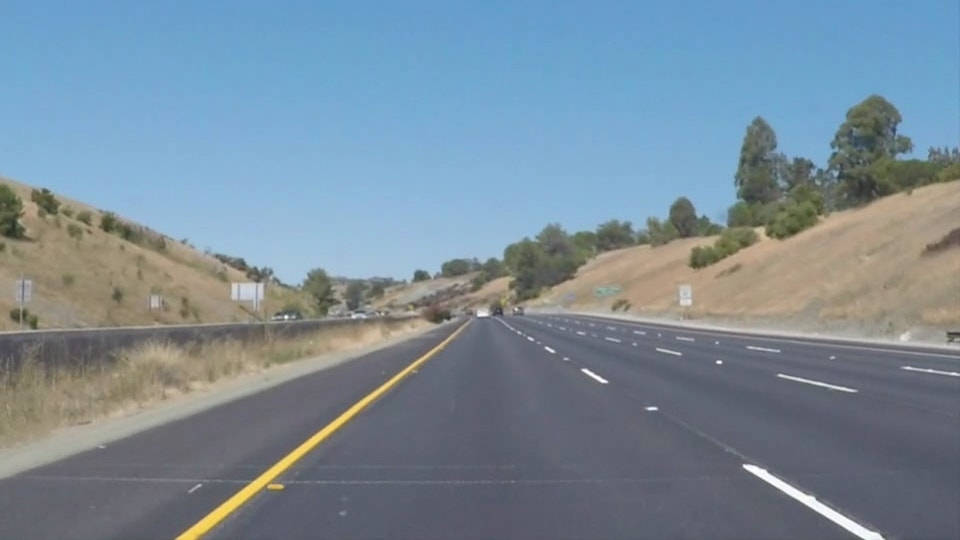
\includegraphics[width=0.8\textwidth]{image}
    \end{subfigure}%
    \begin{subfigure}{0.33\textwidth}
    \centering
    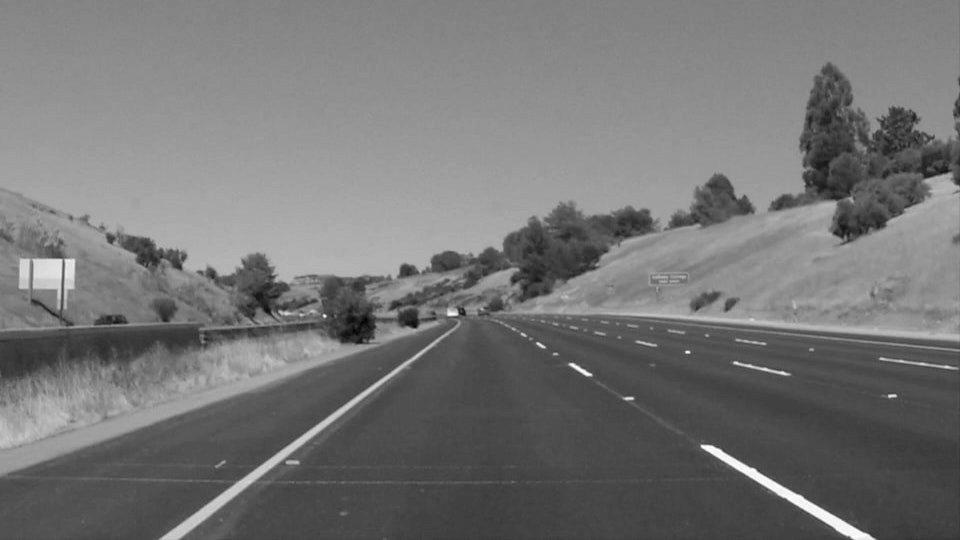
\includegraphics[width=0.8\textwidth]{gray}
    \end{subfigure}%
    \begin{subfigure}{0.33\textwidth}
    \centering
    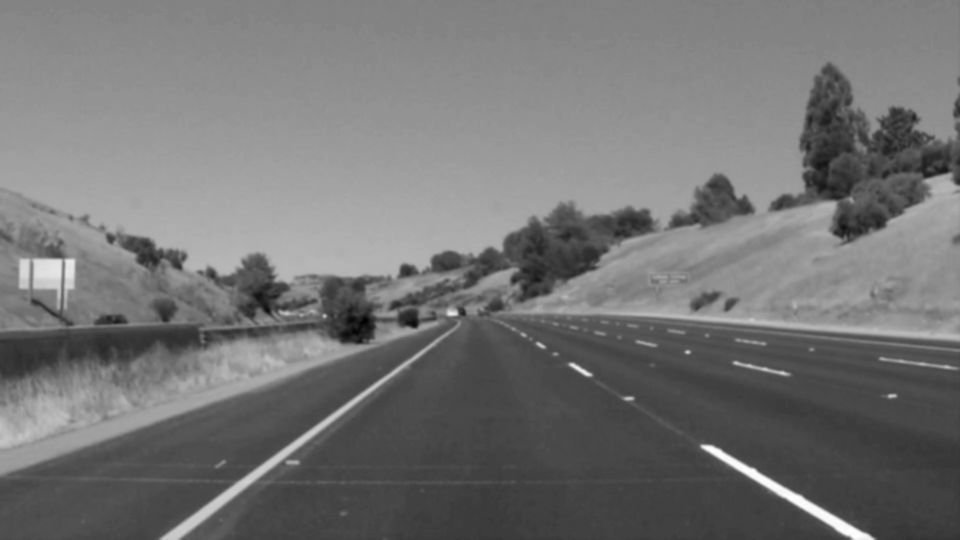
\includegraphics[width=0.8\textwidth]{blurgray}
    \end{subfigure}
    \vspace{3em}
    
    \begin{subfigure}{0.33\textwidth}
    \centering
    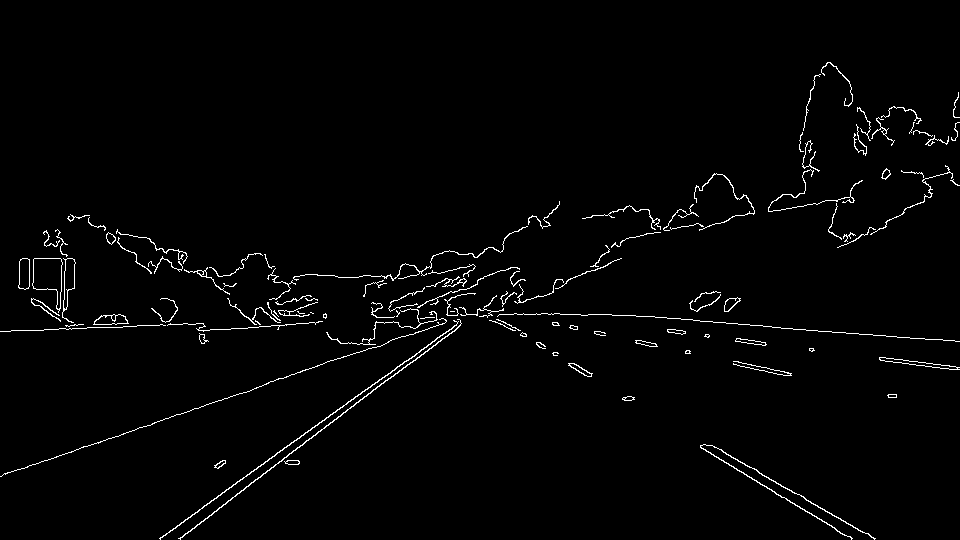
\includegraphics[width=0.8\textwidth]{edges}
    \end{subfigure}%
    \begin{subfigure}{0.33\textwidth}
    \centering
    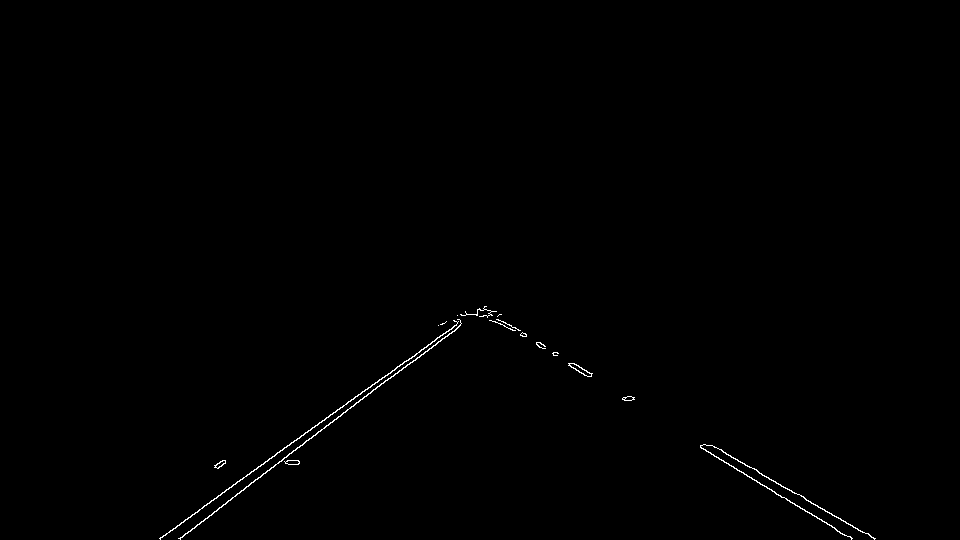
\includegraphics[width=0.8\textwidth]{maskededges}
    \end{subfigure}%
    \begin{subfigure}{0.33\textwidth}
    \centering
    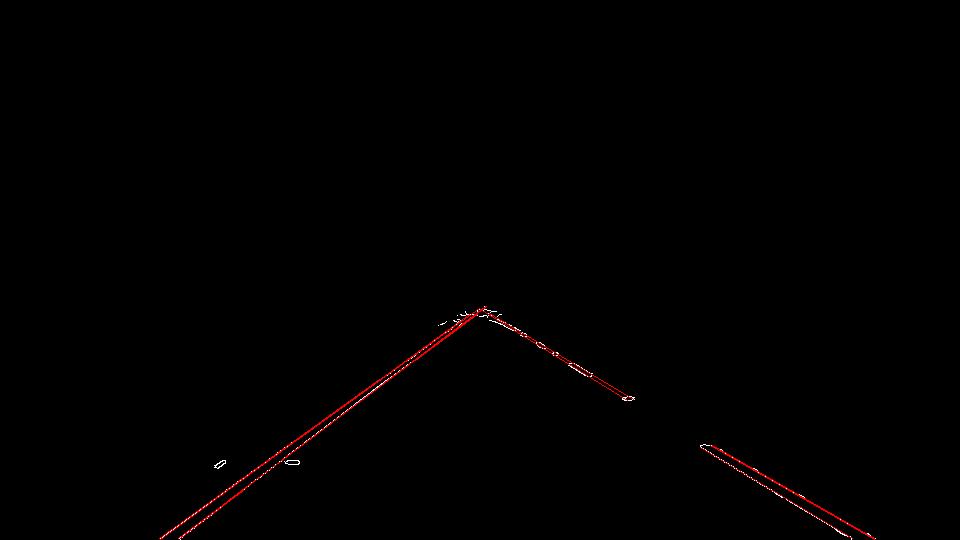
\includegraphics[width=0.8\textwidth]{maskedhough}
    \end{subfigure}
\end{figure}

The Hough line transform simply makes a grid of lines passing through the image, and counts up the number of indicator pixels from Canny that land on those lines. You can define a threshold for the number of votes a line gets before being counted as a line, along with some other variables to affect your line quantity and length.  

\subsection{Obtaining lane lines: segmenting, extrapolating, and averaging segments}

The next task was to figure out a way to average the lane lines to produce a solid line for each lane. The process I chose began with segmenting the lane lines on the right to left side. We'll stick with talking about the left lane for simplicity. This was a simple process of guessing a slope $m$ for the lane and defining a threshold $d\!m$ above and below the slope; any line segments with slopes falling between $[m-d\!m, m+d\!m]$ were included into the left lane category. Then, simply averaging the points and slopes of those lines gives an average line passing close to all of them. Once this average line is constructed, we can simply pass in the $y$ values we want the lanes to start and end at, and obtain the $x$ values that lie at those points. Finally, we have the two endpoints of an approximation to the lane line, and we can then draw them on the image. 

\begin{figure}[htb!]
    \centering
    \caption{Hough Lines to Lane Annotations}
    
    \begin{subfigure}{0.5\textwidth}
    \centering
    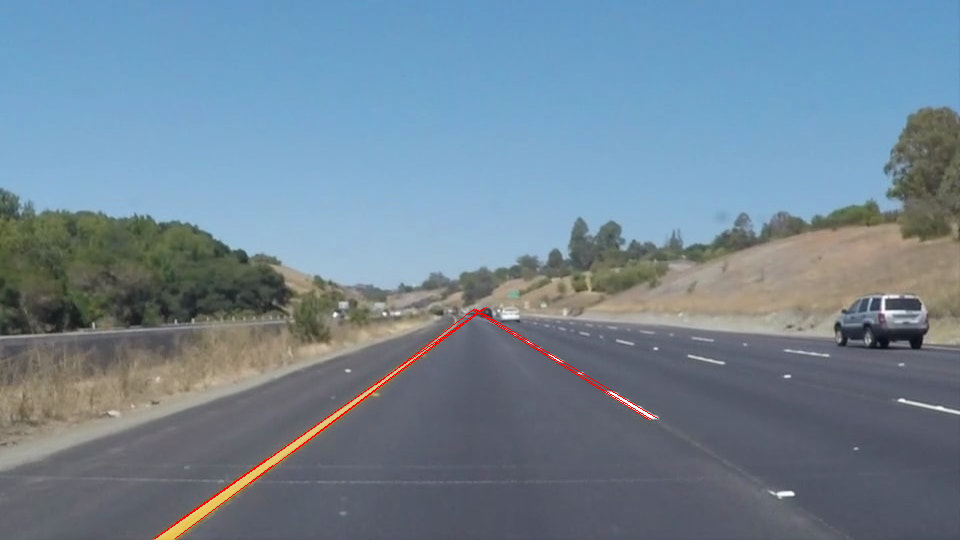
\includegraphics[width=0.8\textwidth]{houghimage}
    \end{subfigure}%
    \begin{subfigure}{0.5\textwidth}
    \centering
    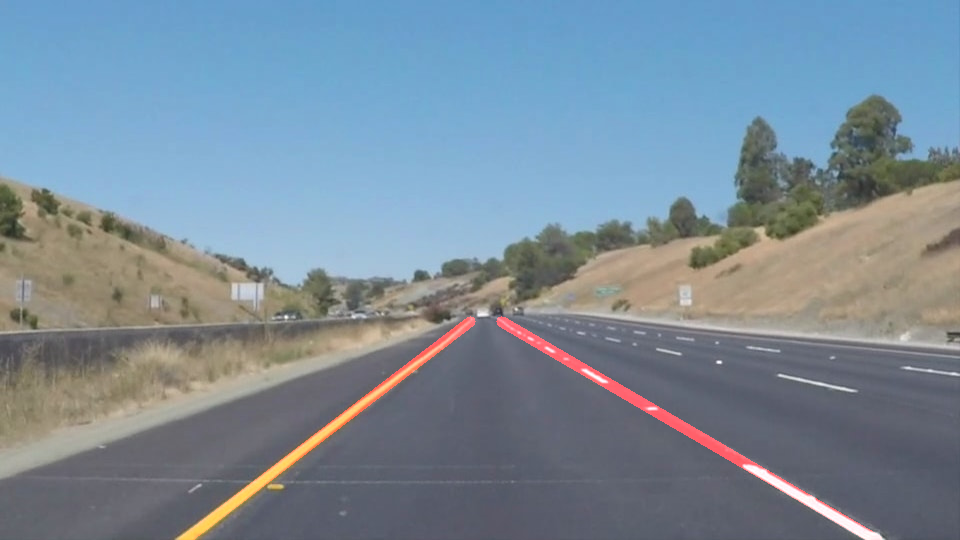
\includegraphics[width=0.8\textwidth]{laneimage}
    \end{subfigure}
\end{figure}


%%%%%%%%%%%%%%%%%%%%%%%%%%%%%%%%%%%%%%%%%%%%%%%%%%%%%%

\section{Video Pipeline}

Applying the image pipeline to the videos gives a decent result, but gives shaky lane lines, and can sometimes fail to produce lane lines for the intermittent passing lanes. Additionally, the natural road bounce can push the lane lines outside of a tight region of interest. Tweaking the settings for Hough can help with the intermittent lines, but not much with the other two issues.

\subsection{Removing lane shakiness: averaging with priors}

If we simply apply the image pipeline, the video feed has no prior knowledge of the frame before, and thus slight deviations are very obvious in the annotated output video. An easy fix is to average the current frame lines with the previous frame lines, and if one of the lanes isn't computed properly, to substitute the prior working lane line. That way, in the next frame that a lane is detected, it can again be averaged with the older working line.

\subsection{Keeping lanes in the mask boundary}

The first frame will need to run on a predefined mask, but the additional frames can only include edges that are near to the lanes from the prior frame. The endpoints of the prior lane are known, so they can be stretched left and right to define a new search area for the edges. That way, if the lanes start to veer or turn, since they do so slowly, the mask follows the lane lines.


%%%%%%%%%%%%%%%%%%%%%%%%%%%%%%%%%%%%%%%%%%%%%%%%%%%%%%

\section{Challenge Video Pipeline}

The challenge video introduced a number of shortcomings to the algorithm. It doesn't account for changes in luminosity between an asphalt and concrete roadway, and additionally, shadows introduce additional edges even in the masked image. The grayscale challenge video shows that the grayscale yellow is very similar to the grayscale concrete roadway, so there needs to be some contrast change to make the yellow pop out from the concrete bridge on the highway.

\begin{figure}[htb!]
    \centering
    \caption{Low contrast lane in grayscale}
    
    \begin{subfigure}{0.5\textwidth}
    \centering
    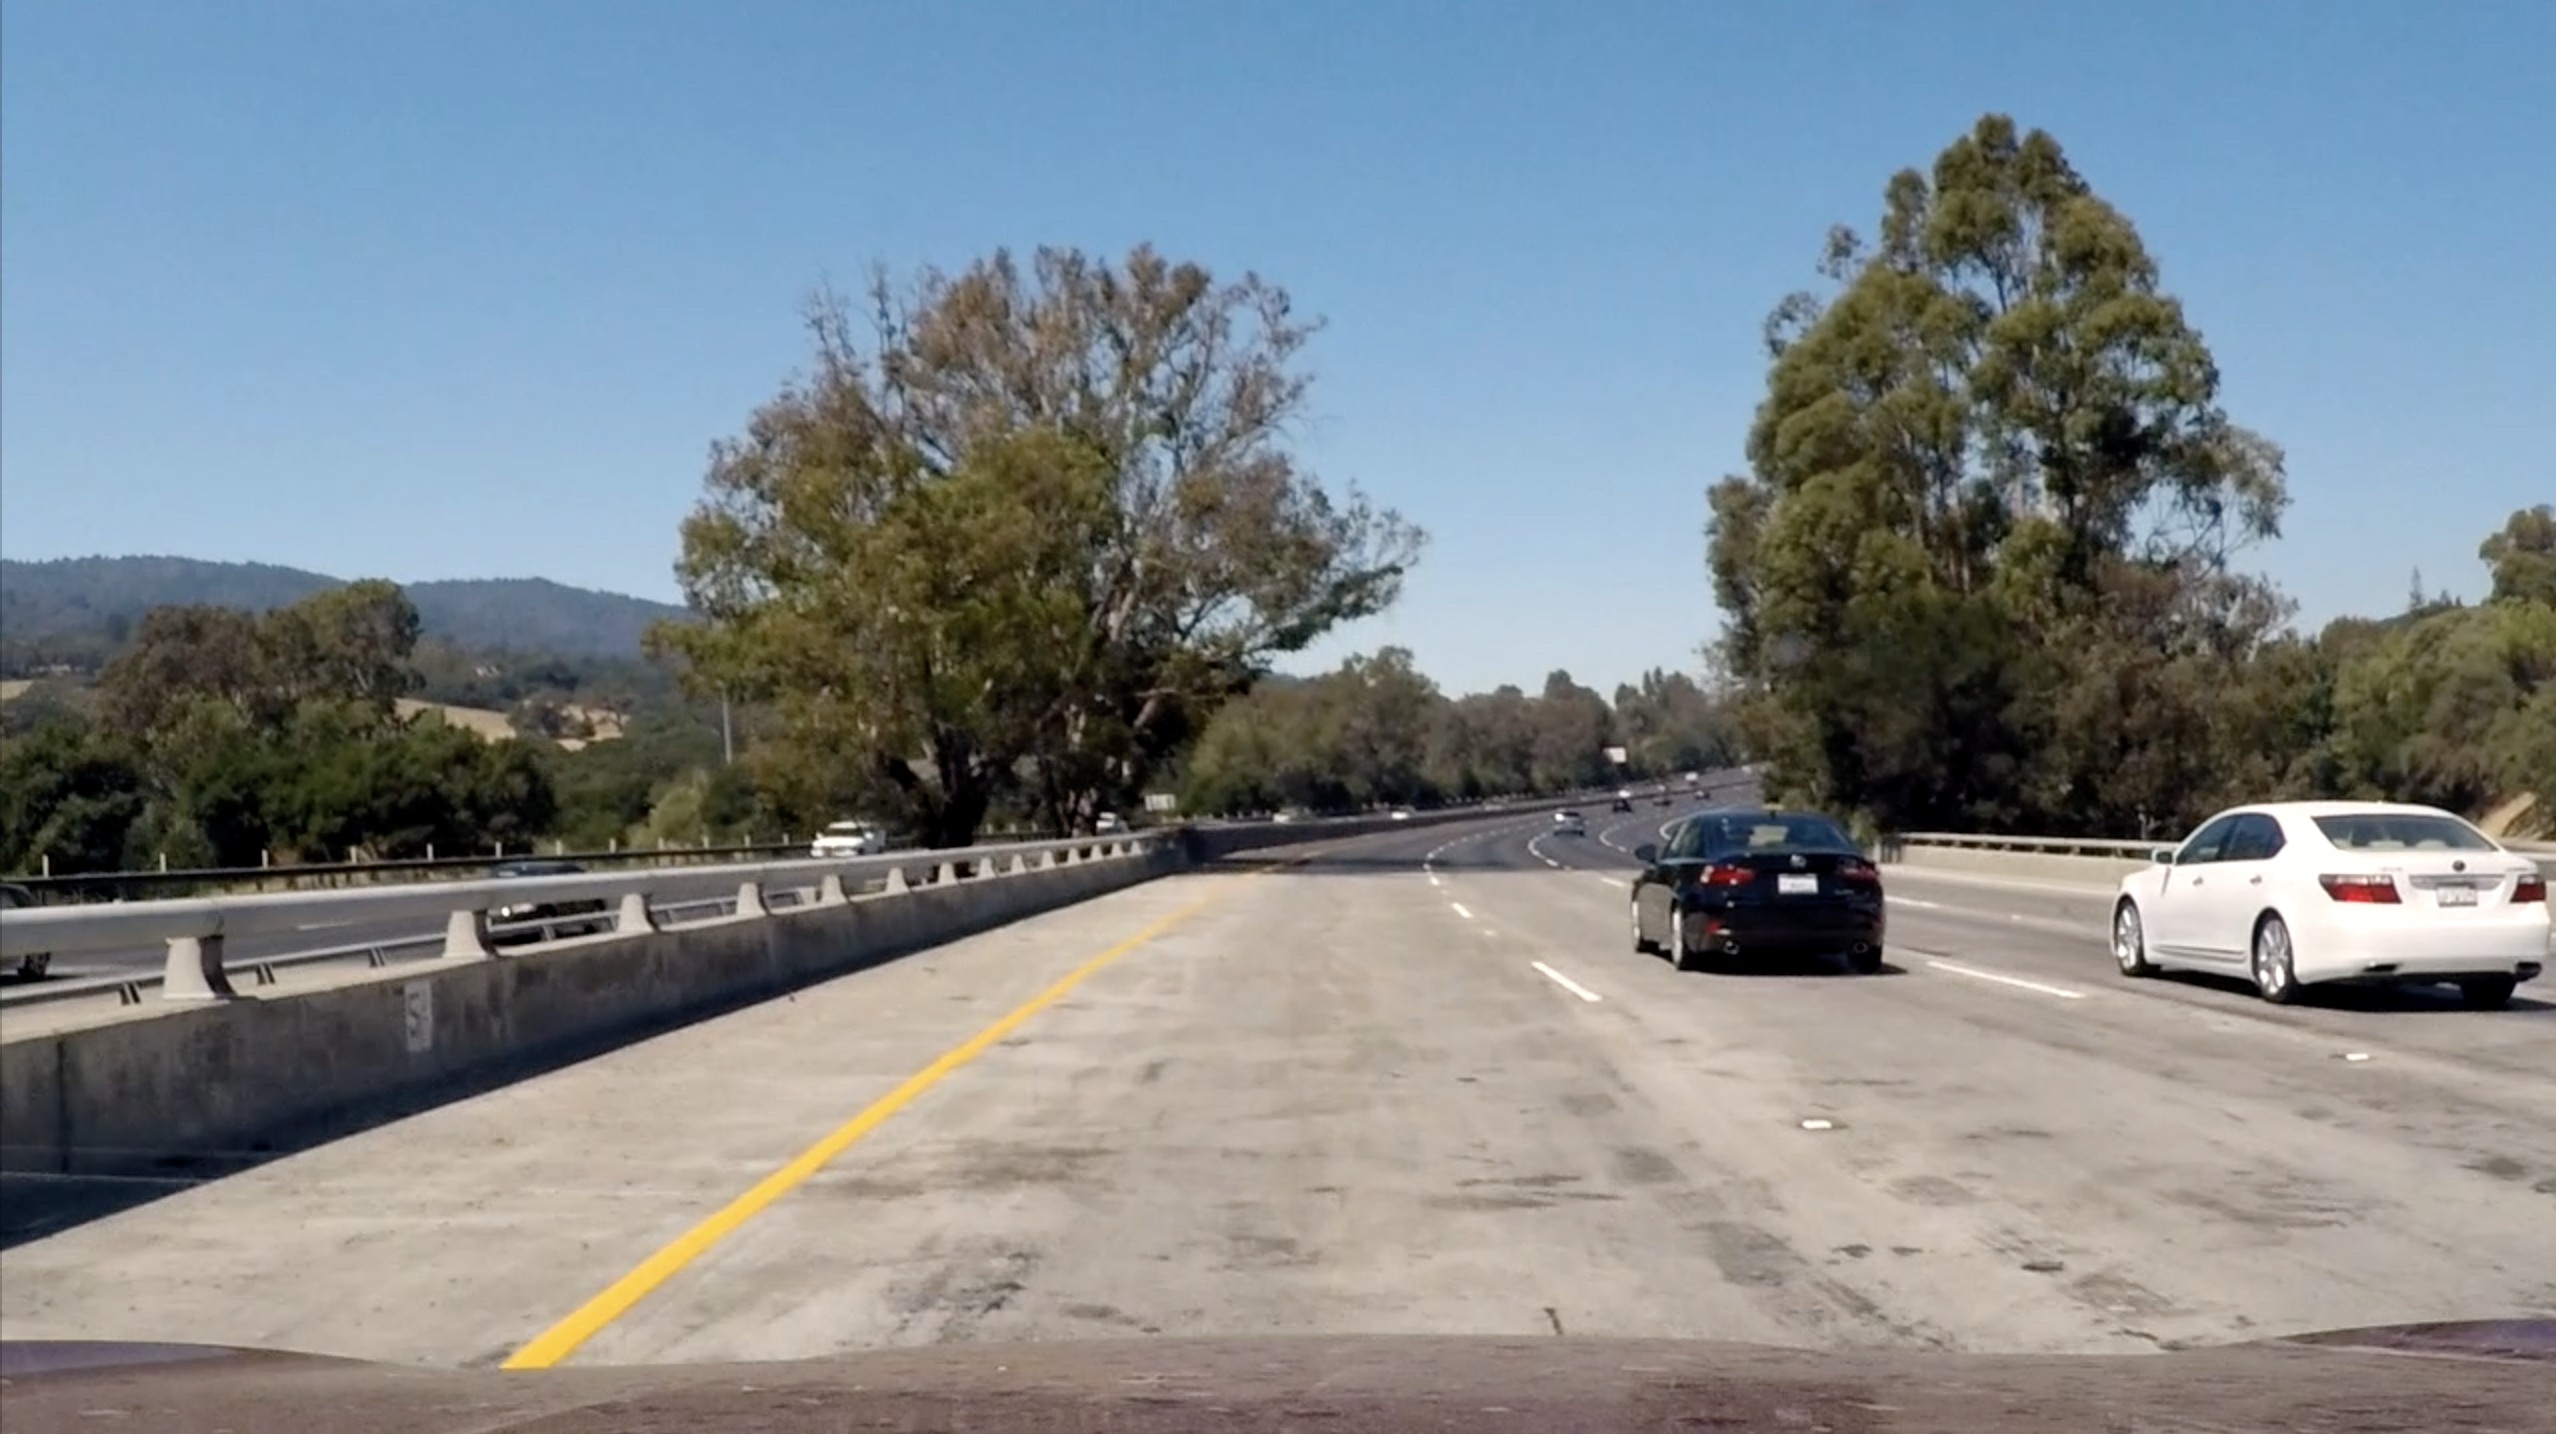
\includegraphics[width=0.8\textwidth]{challenge}
    \end{subfigure}%
    \begin{subfigure}{0.5\textwidth}
    \centering
    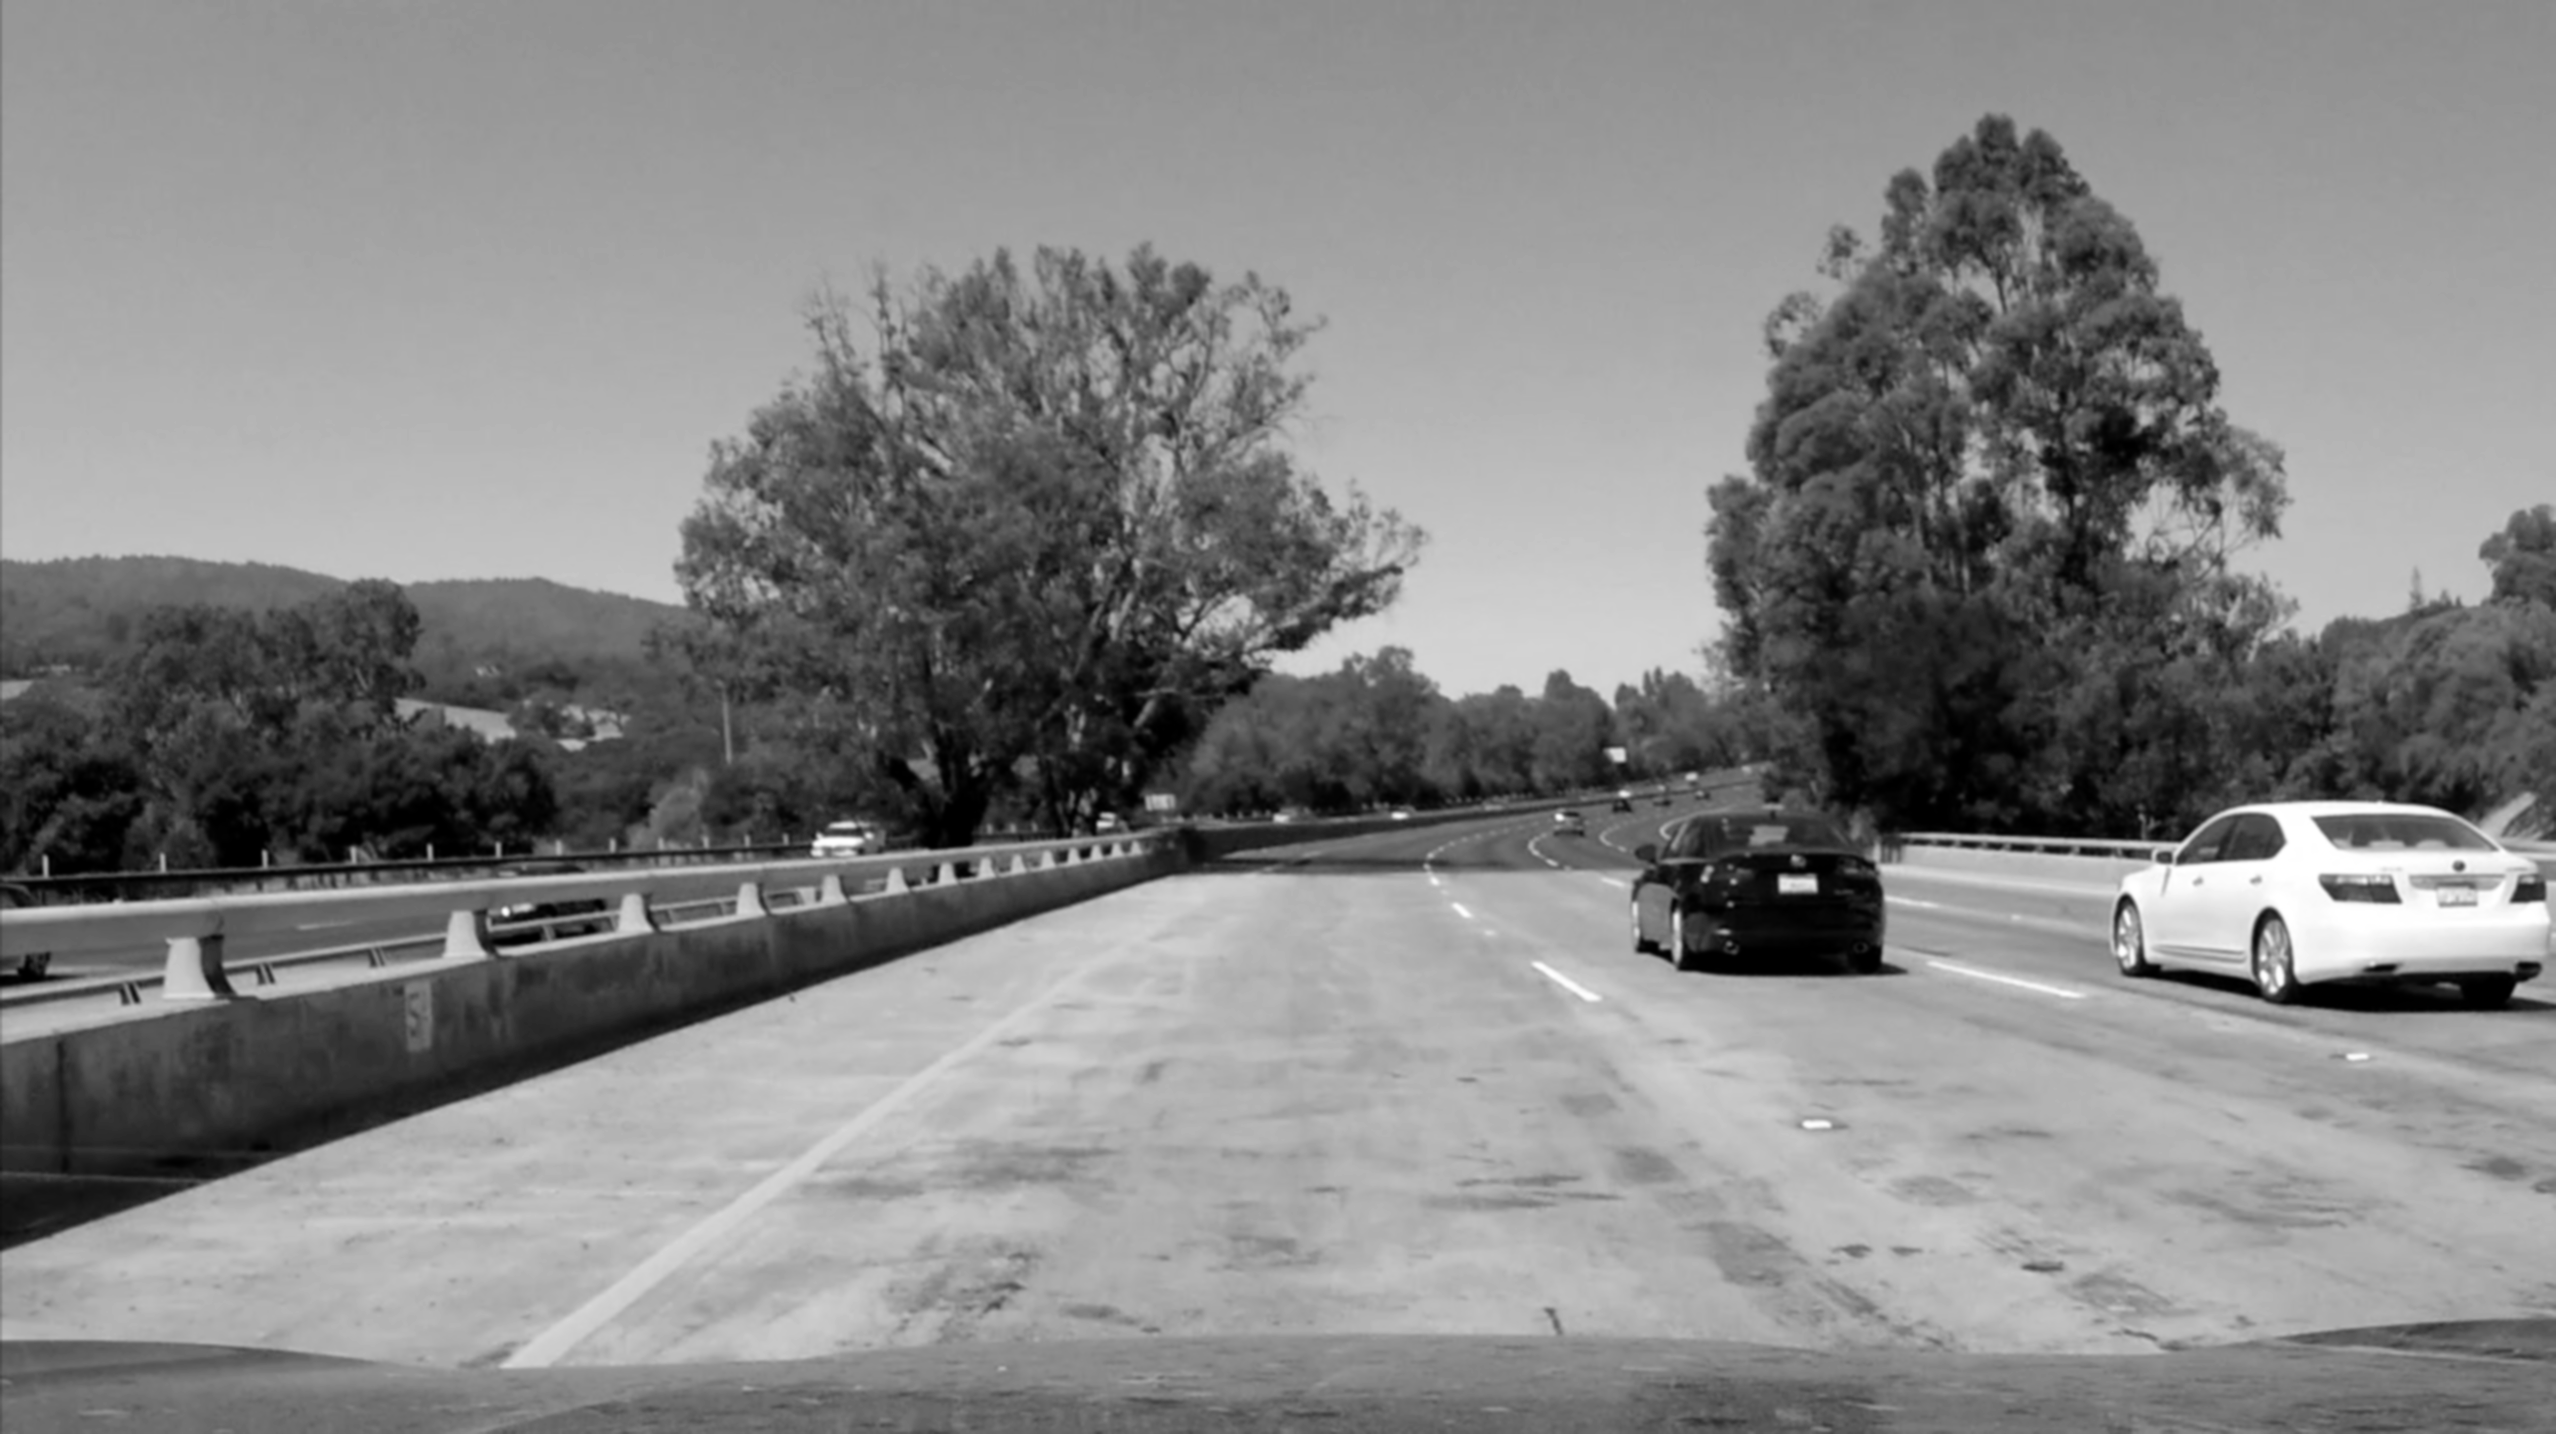
\includegraphics[width=0.8\textwidth]{grayorig}
    \end{subfigure}
\end{figure}

\subsection{Low-contrast lanes: color selection and dilation}

There are a number of ways to increase contrast, but I chose a unique strategy to produce edges on the yellow lane lines. My pipeline selects the yellow in the frame within a certain range, creates an indicator mask for the yellow pixels, then dilates that mask to make sure neighboring yellow pixels are selected. Then the image is made grayscale and ran through the original pipeline.

\begin{figure}[htb!]
    \centering
    \caption{Yellow selection and dilation to improve lane contrast}
    
    \begin{subfigure}{0.5\textwidth}
    \centering
    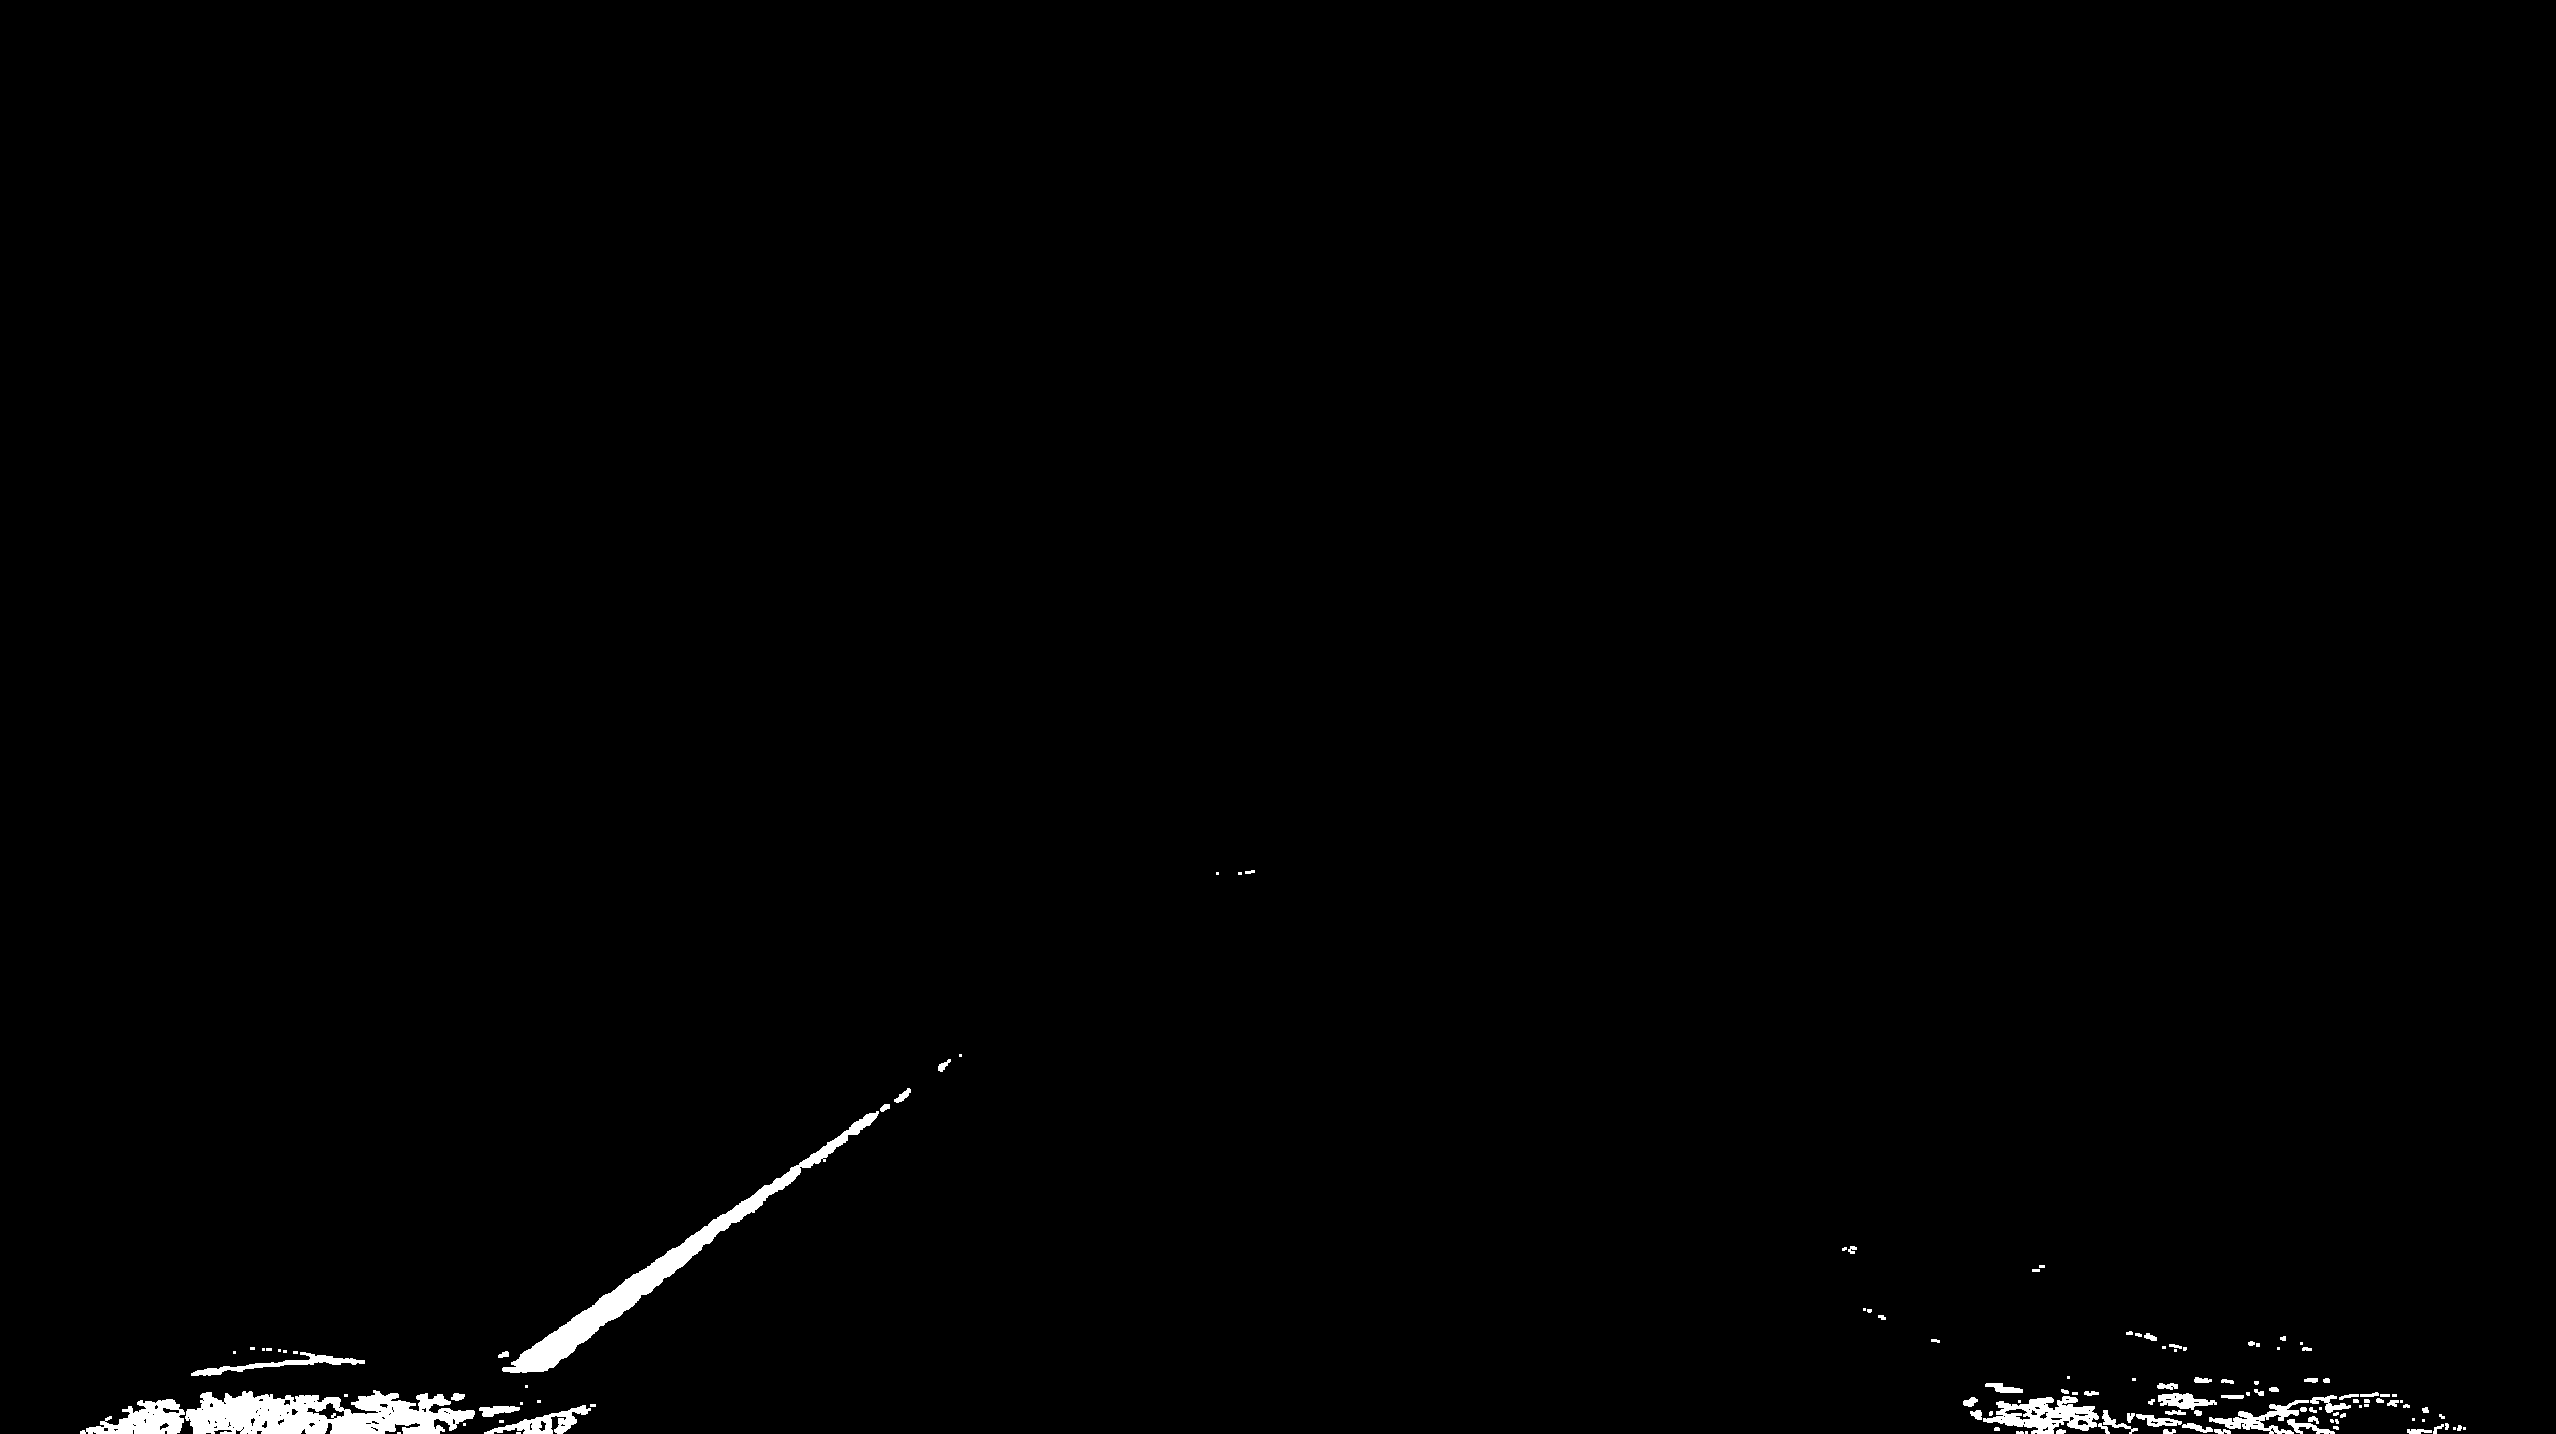
\includegraphics[width=0.8\textwidth]{yellowdilate}
    \end{subfigure}%
    \begin{subfigure}{0.5\textwidth}
    \centering
    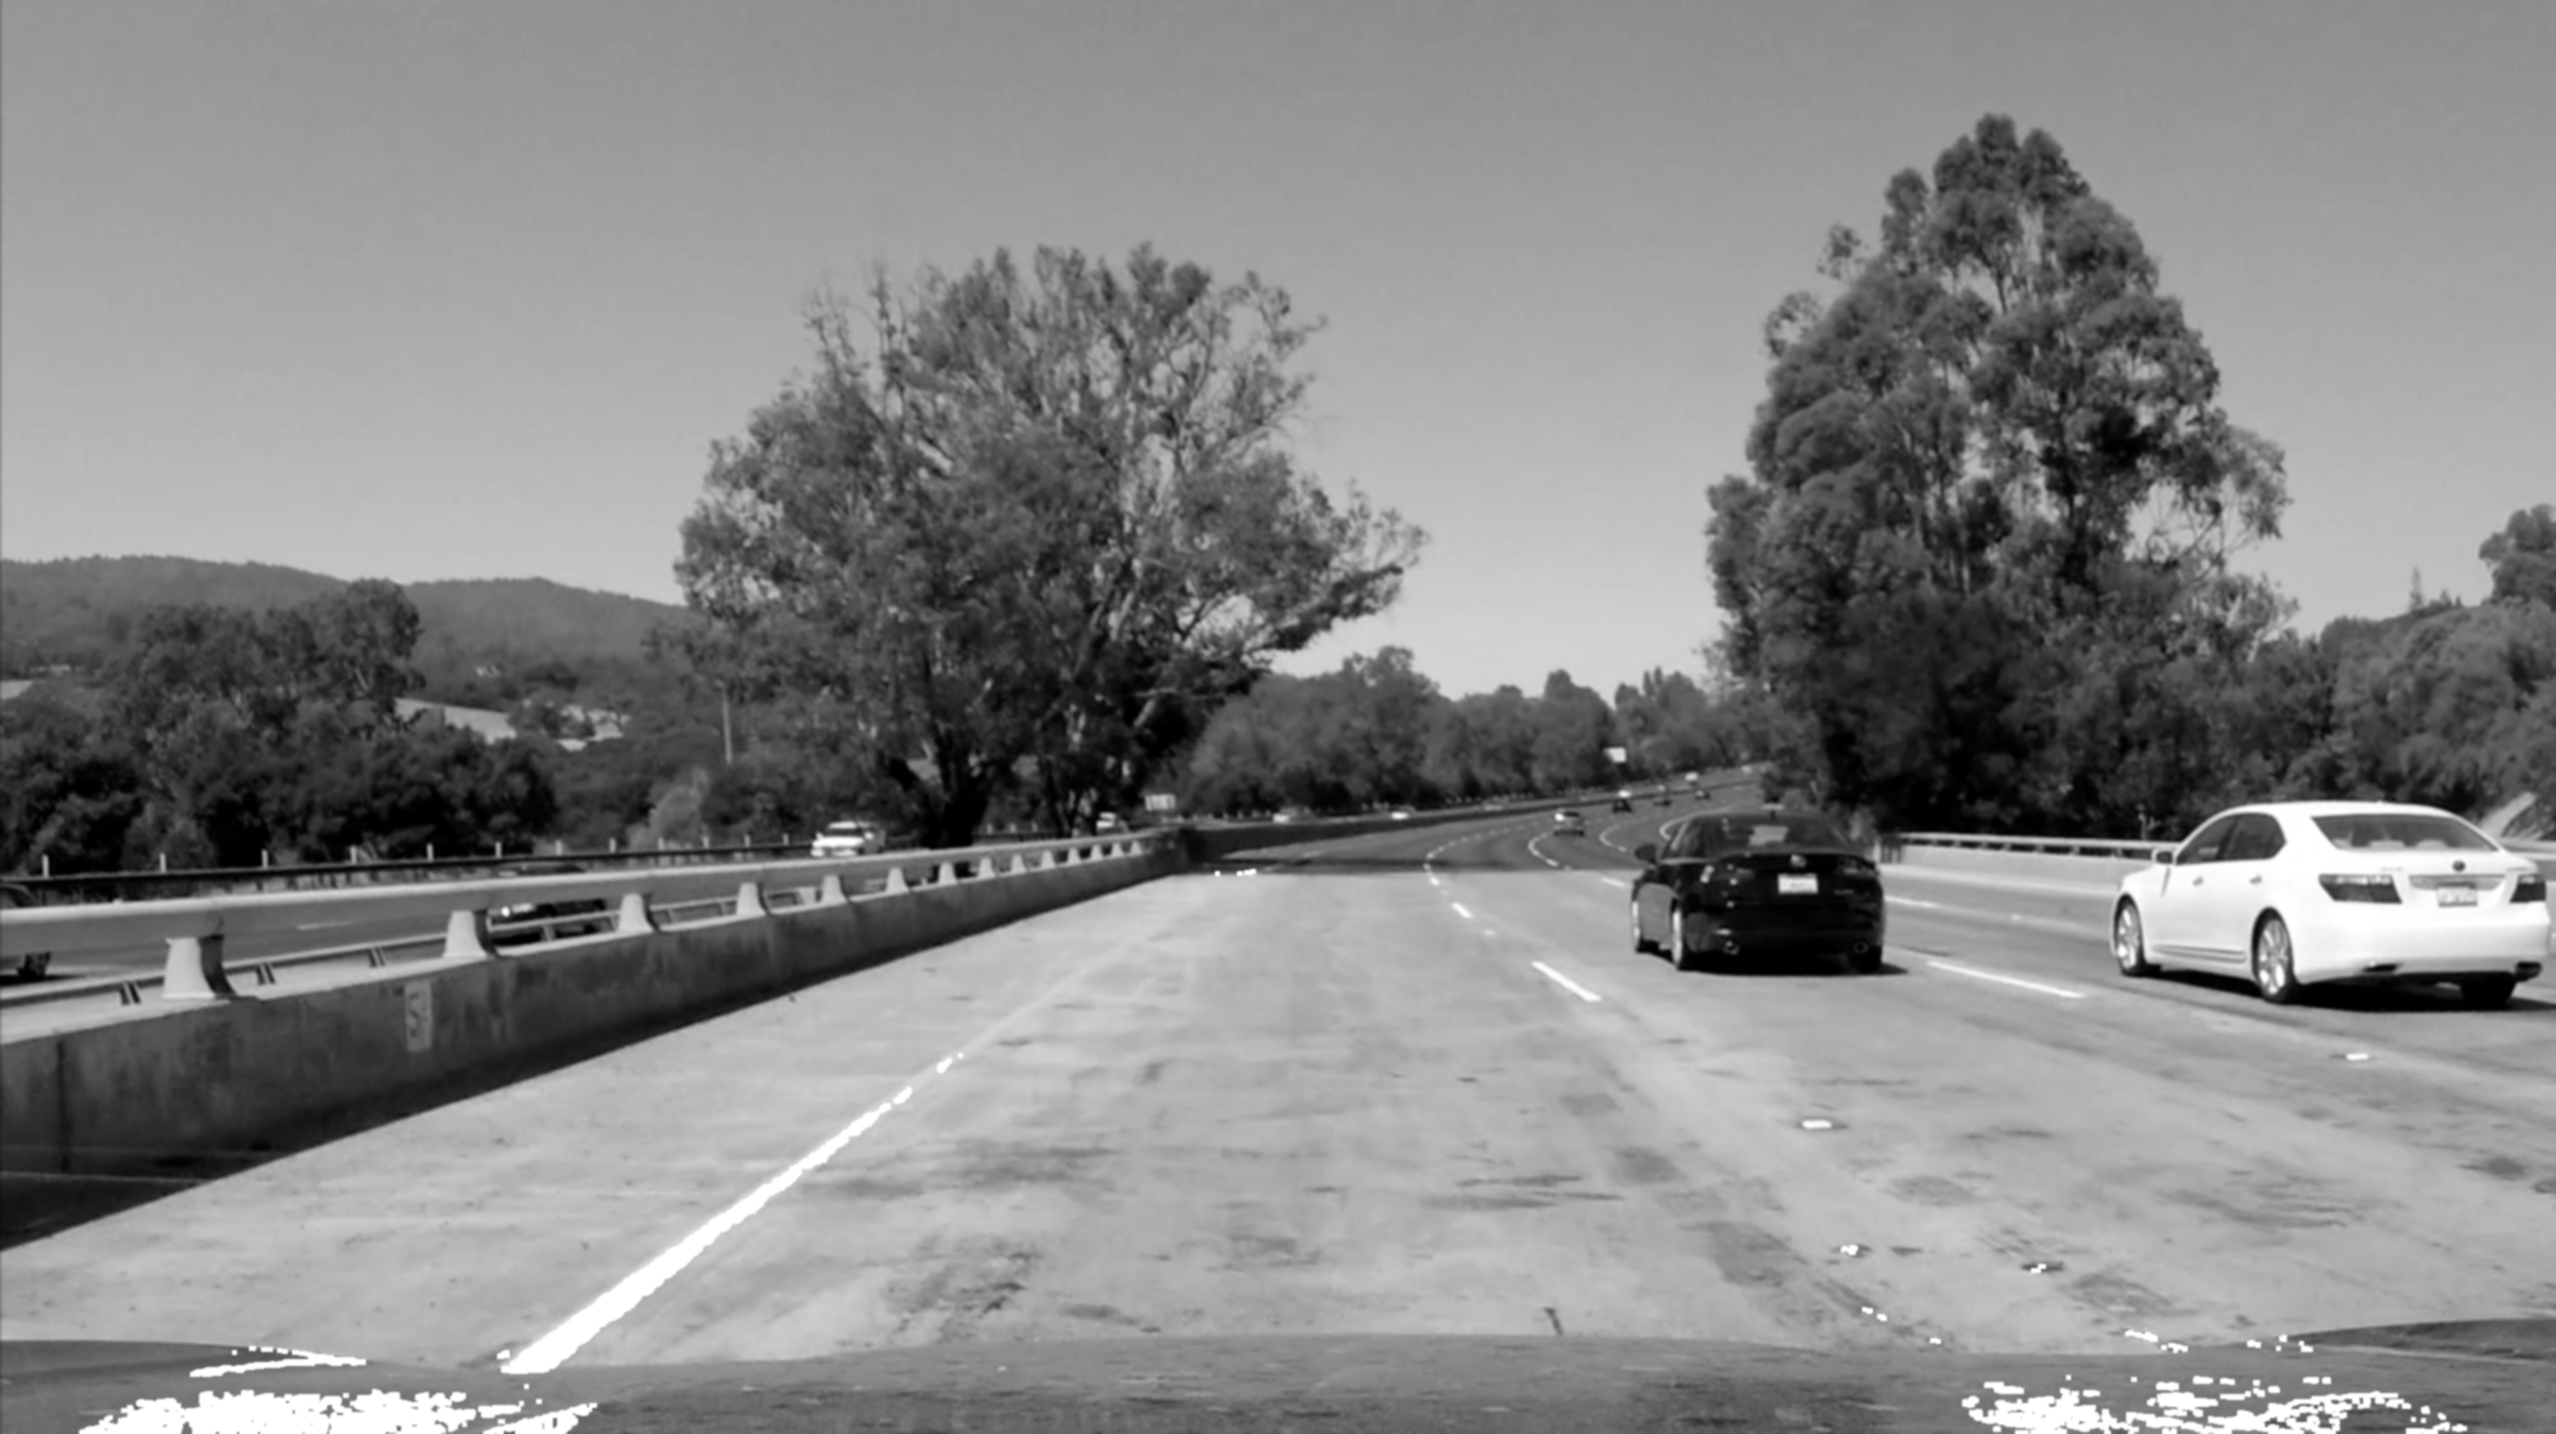
\includegraphics[width=0.8\textwidth]{graydilate}
    \end{subfigure}
\end{figure}

%%%%%%%%%%%%%%%%%%%%%%%%%%%%%%%%%%%%%%%%%%%%%%%%%%%%%%

\section{Extra Challenge Video Pipeline: GoPro}

I decided to take it up one notch by creating my own footage and testing the pipeline. I used a GoPro Hero 4 suctioned to my windshield to take some footage driving in Arizona. I tried to use a challenging part of my video to attempt the algorithm on.

\begin{figure}[htb!]
    \centering
    \caption{GoPro Annotated Line}
    
    \begin{subfigure}{0.5\textwidth}
    \centering
    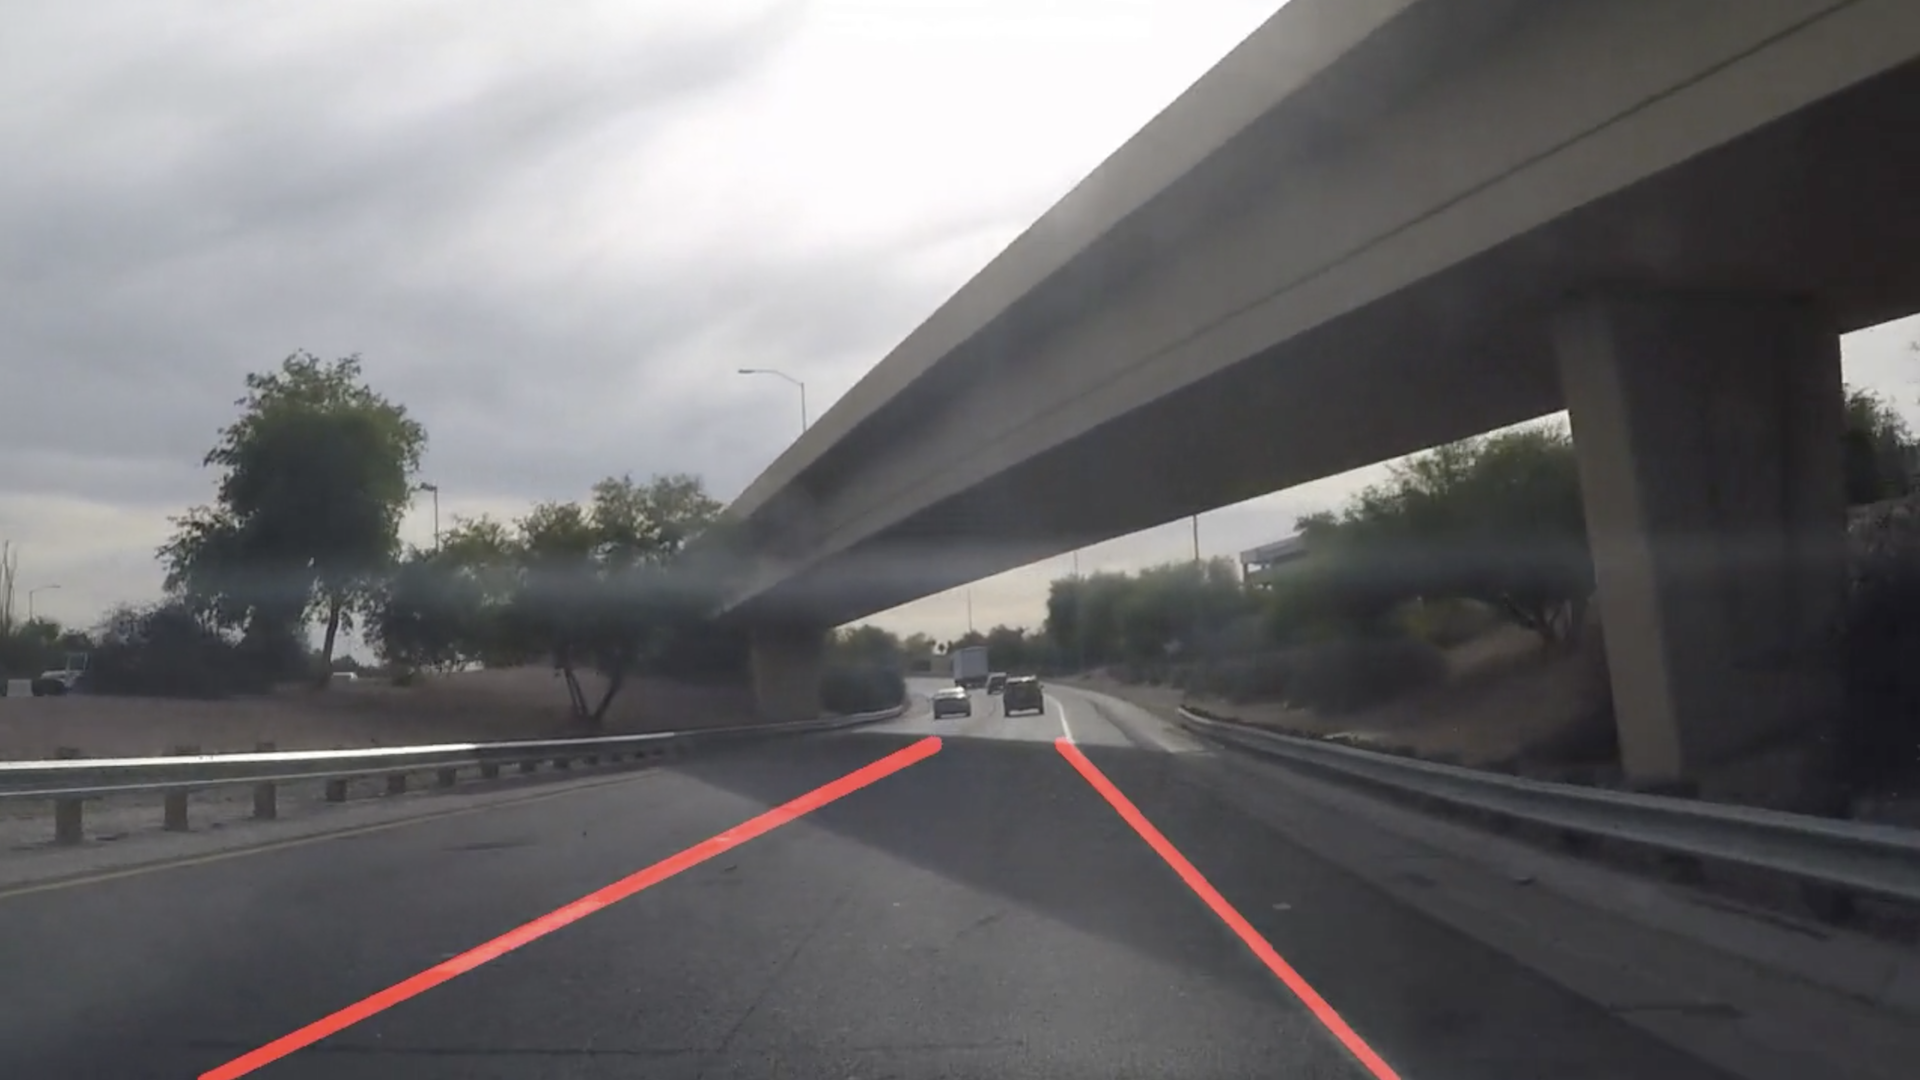
\includegraphics[width=0.8\textwidth]{gopro}
    \end{subfigure}%
\end{figure}

All in all it worked well on the footage, although the automatic light adjustment and dark shadows produced no lines on a couple frames. I had to strongly adjust the original region of interest for the mask and play with the Hough parameters a lot since the contrast and vibrancy is way lower from the raw footage.



%%%%%%%%%%%%%%%%%%%%%%%%%%%%%%%%%%%%%%%%%%%%%%%%%%%%%%

\section{Shortcomings and Improvements}

There are many possible shortcomings of this pipeline, and I will split them into two main categories: shortcomings of the methods used and time-complexity shortcomings.

\subsection{Pipeline shortcomings and improvements}

This pipeline creates lane lines by averaging the detected Hough line segment points. However, this is not a particularly robust method for figuring out a best-fit line for the detected line segments. Instead, linear regression should probably be used, and possible weightings with the length of the detected line \textit{or} weighting by the number of votes in the Hough algorithm; that way, longer or more definite segments contribute stronger to the linear regression line. Since nearer lines to the car are going to be longer and have more Hough votes, this means the region around the car will have the most accurate representation of the lanes.

This pipeline smooths out lane jitter by averaging the current lane with the previous lane. However, the prior lane was also an average. Effectively, if the lane $\ell_n$ in frame $n$ is averaged with the lane $\ell_{n-1}$ from the prior frame $n-1$, then it's actually a weighted average with \textit{all} prior lanes: $\ell_n = \sum_{k=1}^n \frac{1}{2}^n \ell_n$. While this works fine for the videos where the lanes stay relatively constant, it does not make sense that the lane positions from two miles ago have \textit{any} affect on the current lane positions, however small that may be.

This pipeline works fine for the videos provided, but will not work on video where the car changes lanes. My algorithm explicitly gives an original guess for the lane line positions and slopes, but this is not robust for any particular starting position on a road. The original mask for the video is defined on priors, for example, knowing that you're between two lines. An improvement could be realized by finding the vanishing points of all the major lines in the image, average them, and only select lines from the Hough transform that actually map close to those vanishing points. This would allow you to detect multiple lanes, and you can define the left and right by which ones have negative and positive slopes.

An additional problem comes with defining the masked region of interest as being around the prior lanes. It's difficult to know \textit{a priori} how wide that mask should be, and if a lane line is not found, it will keep searching in the same area when the lane line may have moved. A more robust solution would include a growth rate so that the masked region of interest for the lane grows until a lane is detected again.

\subsection{Complexity shortcomings and improvements}

The original Hough transform---not used in this project---searches through all indicator points from Canny and counts the votes. This is very computationally expensive. Instead, this project uses the \textit{probabilistic} Hough transform which uses a random subset of the indicator pixels to find the lines. This means that you get line segments instead of lines through the whole image, which is great, but it is still creating a large matrix of values for the possible lines to search through, and this isn't necessary when we know, for example, that horizontal lines should not be counted as lanes. A computationally robust function would run the probabilistic Hough transform, but only on a small subset of possible parameter values near the prior lanes.

\subsection{Vanishing point detection}

Twenty years ago, a paper was published by Tuytelaars, \textit{et al.}, titled ``The cascaded Hough transform'', which shows the use of repeated iterations of the Hough transform to find signatures in the Hough transform itself leading to the detection of interesting visual cues. One application is the detection of vanishing points and horizon lines in an image. Detection of vanishing points and the lines leading to it can help establish all lane lines in view, and help determine the correct region to mask and figure out which pair of lanes your car is currently in.

\end{document}